\documentclass{jsarticle}
\usepackage[dvipdfmx]{graphicx}
\begin{document}

\title{固体電子構造特論レポート}
\author{1518511 川瀬 拓実}
\maketitle

\newpage

\section{問1 平均のクーロン相互作用の導出}

\[
\overline{U} = \frac{1}{9} (U + 8U^{\prime} - 4J_H)  
\]

電子数が4つなので、10個の軌道から4つ選ぶのは${}_{10} \mathrm{C} _4 = 210$通りある。
電子の状態各々について、エネルギーを足し合わせ、平均のクーロン相互作用を求める。
アップスピンに着目すると、4つ全てがアップスピンの場合、3つがアップスピンの場合、2つがアップスピンの場合、1つのみがアップスピンの場合、1つもアップスピンが存在しない場合が存在するが、対称性から4つがアップスピンの場合と、3つがアップスピンの場合をそれぞれ2倍した場合と2つがアップスピンの場合を考えればいいことがわかる。

\paragraph{↑↑↑↑の場合}
\mbox{}\\
 全てがアップスピンの場合、同一軌道に入ることはないので、5つの軌道から4つを選ぶ場合の数とすると${}_{5} \mathrm{C} _4 = 5$通りとなる。この場合のクーロン相互作用は$(6U^{\prime}-6J_H)$で、和は$5 \times (6U^{\prime} - 6J_H)$となる。

\paragraph{↑↑↑↓の場合}
\mbox{}\\
 3つがアップスピンの場合、まず5つの軌道から3つを選ぶ場合の数なので${}_{5} \mathrm{C} _ 3 = 10$通りとなる。ここでダウンスピン1つの入れ方により、2つの場合に分かれる。

\subparagraph{↓が↑と同じ軌道に入る場合}
\mbox{}\\
 3つのアップスピンどれかと同じ軌道に入る場合の数なので${}_{3} \mathrm{C} _ 1 = 3$から、合計で$10 \times 3 = 30$通りとなる。この場合のクーロン相互作用は$(U+5U^{\prime}-3J_H)$で、和は$30 \times (U+5U^{\prime}-3J_H)$となる。

\subparagraph{↓が↑と異なる軌道に入る場合}
\mbox{}\\
 残り2つの軌道のどちらかに入る場合の数なので${}_{2} \mathrm{C} _ 1 = 2$から、合計で$10 \times 2 = 20$通りとなる。この場合のクーロン相互作用は$(6U^{\prime}-3J_H)$で、和は$20 \times (6U^{\prime}-3J_H)$となる。

\paragraph{↑↑↓↓の場合}
\mbox{}\\
 2つがアップスピンの場合、まず5つの軌道から2つを選ぶ場合の数なので${}_{5} \mathrm{C} _ 2 = 10$通りとなる。ここでダウンスピン2つの入れ方により、3つの場合に分かれる。

\subparagraph{2つの↓が↑と同じ軌道に入る場合}
\mbox{}\\
 2つのアップスピンの場所が決まれば、残り2つのダウンスピンの場所は自動的に決まるので${}_{2} \mathrm{C} _ 2 = 1$から、合計で$10 \times 1 = 10$通りとなる。この場合のクーロン相互作用は$(2U + 4U^{\prime} - 2J_H)$で、和は$10 \times (2U + 4U^{\prime} - 2J_H)$となる。

\subparagraph{1つの↓が↑と同じ軌道に入り、もう1つの↓が↑と異なる軌道に入る場合}
\mbox{}\\
 2つのアップスピンに対して、片方がアップスピンどちらかと同じ軌道、もう片方がアップスピンのない軌道を選ぶ場合の数なので${}_{2} \mathrm{C} _ 1 \times {}_{3} \mathrm{C} _3 = 6$から、合計で$10 \times 6 = 60$通りとなる。この場合のクーロン相互作用は$(U + 5U^{\prime} - 2J_H)$で、和は$60 \times (U + 5U^{\prime} - 2J_H)$となる。

\subparagraph{2つの↓が↑と異なる軌道に入る場合}
\mbox{}\\
 2つのアップスピンが入っていない軌道から2つ選ぶ場合の数なので${}_{3} \mathrm{C} _ 2 = 3$から、合計で$10 \times 3 = 30$通りとなる。この場合のクーロン相互作用は$(6U^{\prime} - 2J_H)$で、和は$30 \times (6U^{\prime} - 2J_H)$となる。

\newpage

以上から、全ての場合についてのクーロン相互作用を足しあげると
\begin{eqnarray}
sum &=& 2 \times 5 \times (6U^{\prime} - 6J_H) + 2 \times 30 \times (U+5U^{\prime}-3J_H) + 2 \times 20 \times (6U^{\prime}-3J_H) + 10 \times (2U + 4U^{\prime} - 2J_H) \nonumber \\
&\quad+& 60 \times (U + 5U^{\prime} - 2J_H) + 30 \times (6U^{\prime} - 2J_H) \nonumber \\
&=&  140U + 1120U^{\prime} - 560J_H \nonumber
\end{eqnarray}
全ての場合の数$210$で割ると、平均のクーロン相互作用$\overline{U}$は
\begin{eqnarray}
\overline{U} &=& \frac{1}{210}(140U + 1120U^{\prime} - 560J_H) \nonumber \\
&=& \frac{2}{3} (U+8U^{\prime}-4J_H) \nonumber
\end{eqnarray}

\section{問2 電子相関ギャップと電荷移動ギャップの導出}

\subsection{電荷移動ギャップの導出}
配位子から電子を受け取った場合の$d$電子系の基底エネルギーは$E_G(d^{n+1}L)=E_G(d^n)+\Delta(n)$と書ける。
これを使うとエネルギーギャップは$ \Delta _{gap} = E_G(d^{n+1})-E_G(d^{n})= \Delta (n)$になる。
さらに多重項補正を取り入れると、Kanamoriの近似から
\begin{eqnarray}
  \Delta _{eff} - \Delta
  = \left\{ \begin{array}{ll}
    n \times (- \frac{7}{9} J_H) & (1 \leq n \leq 4) \\
    n \times (- \frac{7}{9} J_H) + 7 J_H & (5 \leq n \leq 9)
  \end{array} \right. \nonumber
\end{eqnarray}

以上から$1 \leq n \leq 9$について電荷移動ギャップを求めると
\begin{eqnarray}
  \Delta _{gap}
  = \left\{ \begin{array}{ll}
    \Delta(n) + n \tilde{J}_H & (1 \leq n \leq 4) \\
    \Delta(n) + (9 - n) \tilde{J}_H & (5 \leq n \leq 9)
  \end{array} \right. \nonumber
\end{eqnarray}
となる。

\subsection{電子相関ギャップ}
$\overline{U}$を$U^{\prime}$と$\tilde{J}_H$を使って表す。
\begin{eqnarray}
  \overline{U} &=& \frac{1}{9} (9U^{\prime} -2J_H) \nonumber \\
  &=& U^{\prime} - \frac{2}{9}J_H \nonumber \\
  &=& U^{\prime} - \frac{2}{7}\tilde{J}_H \nonumber
\end{eqnarray}
これを使って電子相関ギャップを書き換えると
\begin{eqnarray}
  U_{gap}(1) &=& \overline{U} - \tilde{J}_H \nonumber \\
  U_{gap}(2) &=& \overline{U} - \tilde{J}_H \nonumber \\
  U_{gap}(3) &=& \overline{U} - \tilde{J}_H + 10Dq \nonumber \\
  U_{gap}(4) &=& \overline{U} - \tilde{J}_H \nonumber \\
  U_{gap}(5) &=& \overline{U} + 8\tilde{J}_H - 10Dq \nonumber \\
  U_{gap}(6) &=& \overline{U} - \tilde{J}_H \nonumber \\
  U_{gap}(7) &=& \overline{U} - \tilde{J}_H \nonumber \\
  U_{gap}(8) &=& \overline{U} - \tilde{J}_H + 10Dq \nonumber \\
  U_{gap}(9) &=& \overline{U} - \tilde{J}_H \nonumber
\end{eqnarray}

\section{$\mathrm{La}M\mathrm{O_3}$における電子相関ギャップと電荷移動ギャップの比較}
\subsection{電荷移動ギャップと電子相関ギャップの導出}
問2で求めた電荷移動ギャップと電子相関ギャップをそれぞれ計算する。\\
\subsubsection{電荷移動ギャップの計算}
\begin{eqnarray}
  \Delta _{gap}
  &=& \left\{ \begin{array}{ll}
    \Delta(n) + n \tilde{J}_H & (1 \leq n \leq 4) \\
    \Delta(n) + (9 - n) \tilde{J}_H & (5 \leq n \leq 9)
  \end{array} \right. \nonumber \\
  &=& \left\{ \begin{array}{ll}
    12 \tilde{J}_H - \tilde{J}_H \Delta _z + n \tilde{J}_H = (12 - \Delta _z + n) \tilde{J}_H & (1 \leq n \leq 4) \\
    12 \tilde{J}_H - \tilde{J}_H \Delta _z + (9 - n) \tilde{J}_H = (21 - \Delta _z -n) \tilde{J}_H & (5 \leq n \leq 9)
  \end{array} \right. \nonumber
\end{eqnarray}
\subsubsection{電子相関ギャップの計算}
\begin{eqnarray}
  U_{gap}(1) &=& (7 + \frac{1}{2} \Delta _z)\tilde{J}_H \nonumber \\
  U_{gap}(2) &=& (7 + \frac{1}{2} \Delta _z)\tilde{J}_H \nonumber \\
  U_{gap}(3) &=& (9 + \frac{1}{2} \Delta _z)\tilde{J}_H \nonumber \\
  U_{gap}(4) &=& (7 + \frac{1}{2} \Delta _z)\tilde{J}_H \nonumber \\
  U_{gap}(5) &=& (14 + \frac{1}{2} \Delta _z)\tilde{J}_H \nonumber \\
  U_{gap}(6) &=& (7 + \frac{1}{2} \Delta _z)\tilde{J}_H \nonumber \\
  U_{gap}(7) &=& (7 + \frac{1}{2} \Delta _z)\tilde{J}_H \nonumber \\
  U_{gap}(8) &=& (9 + \frac{1}{2} \Delta _z)\tilde{J}_H \nonumber \\
  U_{gap}(9) &=& (7 + \frac{1}{2} \Delta _z)\tilde{J}_H \nonumber
\end{eqnarray}

\newpage

\subsection{}
$\Delta, \overline{U}, \Delta_{gap}, U_{gap}$をグラフに図示すると以下のようになる。($\Delta _z = 0$とした。) \\
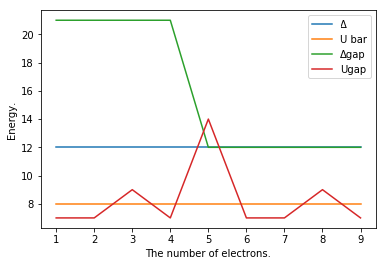
\includegraphics[width=10cm]{graph01.png}

\section{LSの場合}
これまでの計算はHSについて行ったので、改めてLSについて計算する必要がある。
\subsection{電荷移動ギャップ}
HSからLSになったことで変わるのは、Kanamoriの近似だと考えられるが、LSの場合のKanamoriの近似が分からなかったので$\Delta _{gap} = \Delta(n)$とする。

\subsection{電子相関ギャップ}


\end{document}
